\documentclass[a4paper,11pt,final]{article}

\usepackage[english,francais]{babel}
\usepackage[utf8]{inputenc}
\usepackage[T1]{fontenc}
\usepackage[pdftex]{graphicx}
\usepackage{setspace}
\usepackage{hyperref}
\usepackage[french]{varioref}
\usepackage{graphicx}

\newcommand{\reporttitle}{Inversion de couleurs} 
\newcommand{\reportauthor}{Valentin \textsc{Durand}} 
\newcommand{\reportsubject}{TPE : Fondements de l'informatique} 
\newcommand{\HRule}{\rule{\linewidth}{0.5mm}}
\setlength{\parskip}{1ex} 
\setlength{\textwidth}{150mm}
\setlength{\oddsidemargin}{5mm}
\setlength{\topmargin}{0mm}
\setlength{\textheight}{220mm}

\hypersetup{
    pdftitle={\reporttitle},%
    pdfauthor={\reportauthor},%
    pdfsubject={\reportsubject}
}

%% Le titre du papier
\title{TPE : \textsc{Fondements de l'informatique \\ Inversion de couleurs}}
\author{Valentin Durand, ENSICAEN -- 1A Informatique (2015-2016)}

\begin{document}
\maketitle

\tableofcontents
\sloppy 
\cleardoublepage

\section*{Introduction}
\addcontentsline{toc}{section}{Introduction}

Ce projet a permis de mettre en pratique les connaissances acquises en programmation C au cours du premier semestre, notamment les structures de données et les allocations dynamiques, afin de produire un programme limitant les couleurs d'une image à celles disponibles dans une table prédéfinie. Ce programme prend en paramètre une image et une table de couleur, puis se charge pour chaque pixel de chercher sa couleur la plus proche dans la table de couleur, de remplacer ce pixel par la couleur trouvée et de sauvegarder l’image finale. L’algorithme de recherche de la couleur la plus proche est décliné en deux versions, une méthode triviale assez lente et une méthode utilisant des arbres binaires afin d’accélérer la durée d’exécution. Ce rapport a donc pour but de détailler l’implémentation de ces deux méthodes et de comparer leurs résultats.

\section{Méthode de travail}

Bien que ce projet ait été réalisé en monôme, un gestionnaire de version a été utilisé afin de structurer le travail à effectuer au cours des mois de décembre et janvier. Les jalons ont suivis linéairement les consignes stipulées dans l’énoncé:
\begin{itemize}
\item Familiarisation avec le module image \emph{(16 Dec)} ;
\item Création du module table de couleur \emph{(16 - 22 Dec)} ;
\item Implémentation de la méthode triviale \emph{(22 Dec - 1 Jan)} ;
\item Construction du kd arbre \emph{(1 - 2 Jan)} ;
\item Calcul de la couleur la plus proche dans l’arbre \emph{(2 Jan)} ;
\item Inversion de couleur par kd arbre \emph{(2 Jan)} ;
\item Comparaison des résultats \emph{(31 Jan)}.
\end{itemize}

\begin{figure}[ht!]
	\centering
	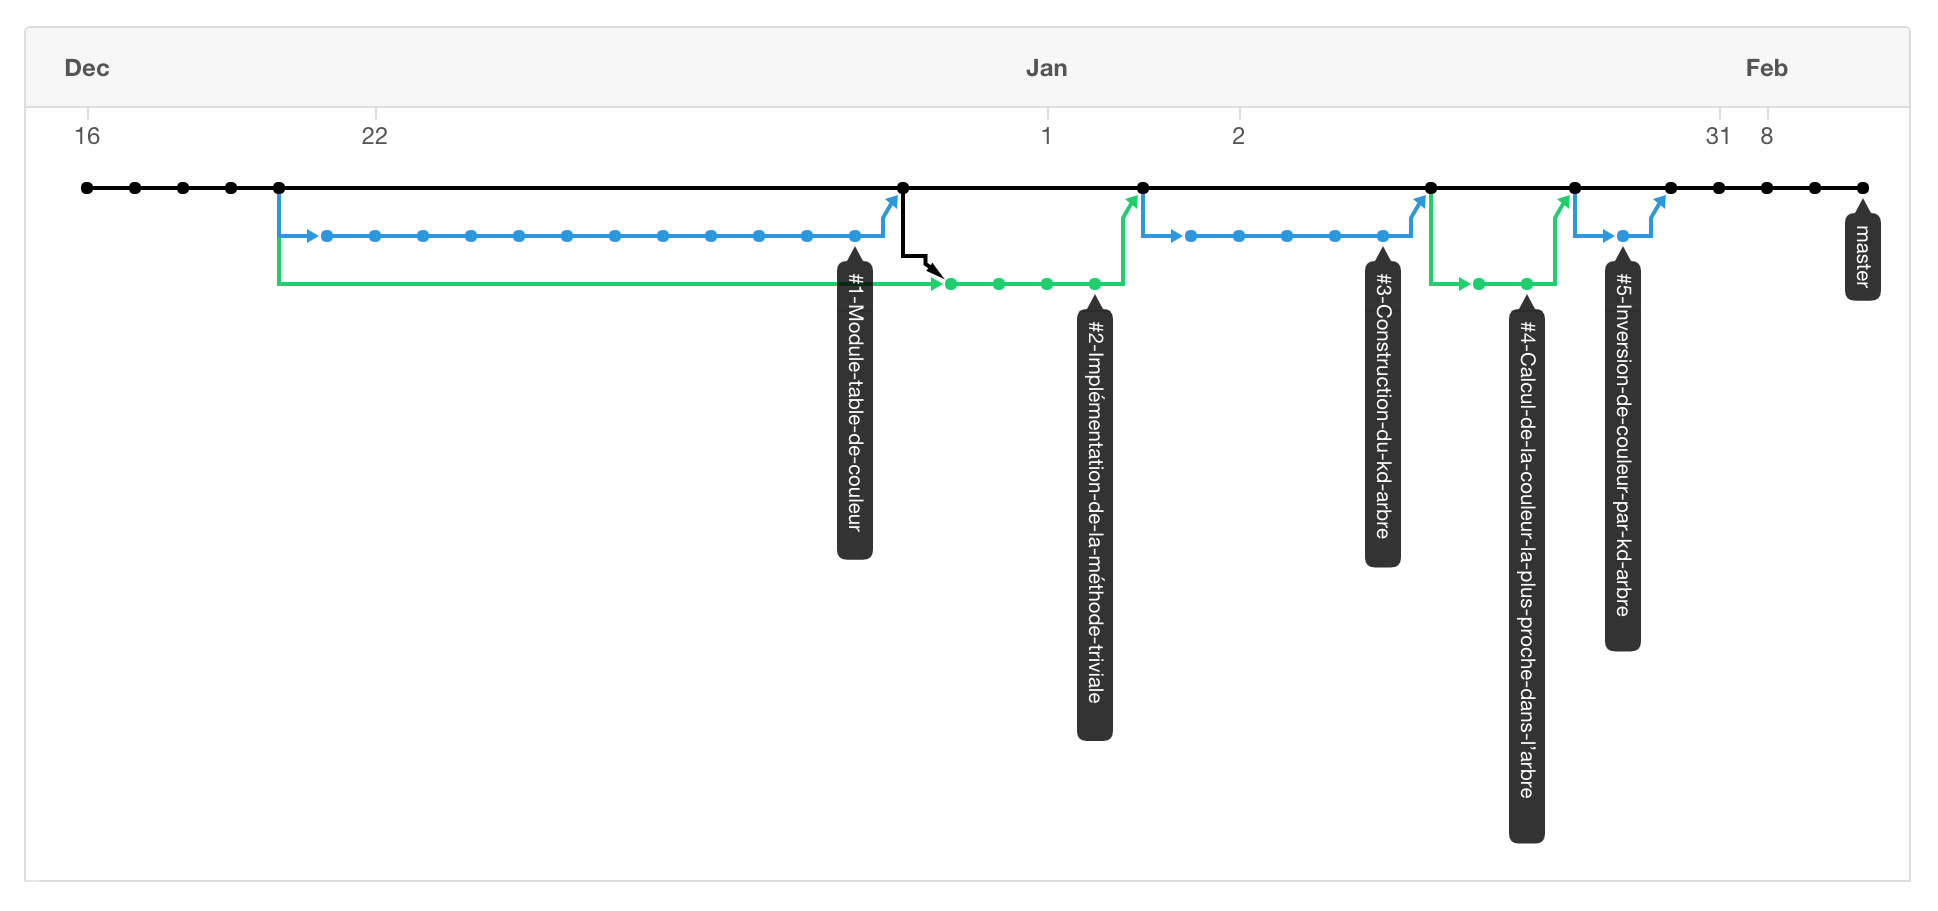
\includegraphics[width=150mm]{./pic/gitTree.jpg}
\end{figure}

L’intégralité des commits sont disponibles à l’adresse suivante: \url{https://github.com/vDurand/ProjetC-Inversion/commits/master}

\section{Architecture}

\begin{figure}[!ht]
    \centering
    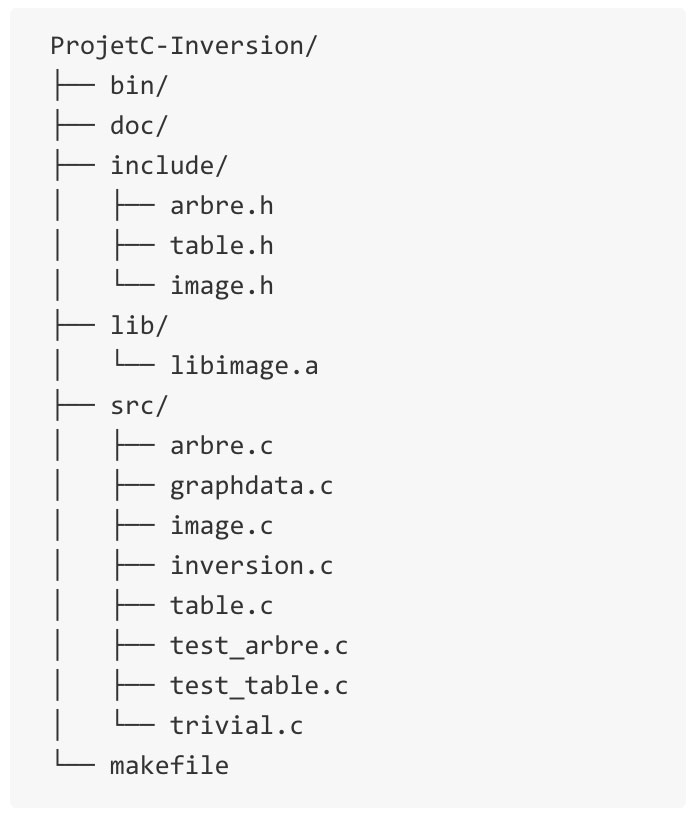
\includegraphics[width=70mm]{./pic/directoryStructure.jpg}
\end{figure}

Afin de gérer les images ppm, le programme exploite le module image sous forme du image.c compilé en librairie statique libimage.a contenu dans le dossier lib. Le makefile permet de compiler trois exécutables:
\begin{itemize}
\item trivial qui réalise l’inversion des couleurs par la méthode trivial ;
\item inversion qui réalise l’inversion des couleurs par le biais d’un kd arbre ;
\item graph data qui permet de générer un fichier contenant les temps nécéssaire pour l’inversion une image par la méthode trivial et la méthode kd arbre avec des tables successivement de 128, 256, 512 et 1024 couleurs.
\end{itemize}

\section{Table de couleur}
\subsection{Structure des données}
\subsection{Fonctions}
\section{Méthode triviale}
\section{Kd arbre}
\subsection{Structure des données}
\subsection{Fonctions}
\section{Conclusion}
\addcontentsline{toc}{section}{Conclusion}

\end{document}